% DySTGAT Presentation
% Dynamic Spectral-Temporal Graph Attention Network for Anomaly Detection
\documentclass[aspectratio=169,11pt]{beamer}

% Theme and colors
\usetheme{Madrid}
\usecolortheme{whale}
\setbeamertemplate{navigation symbols}{}
\setbeamertemplate{footline}[frame number]

% Packages
\usepackage{tikz}
\usepackage{pgfplots}
\usepackage{booktabs}
\usepackage{multirow}
\usepackage{amsmath,amssymb}
\usepackage{algorithm}
\usepackage{algorithmic}
\usepackage{xcolor}
\usepackage{subcaption}

% TikZ libraries
\usetikzlibrary{shapes,arrows,positioning,fit,calc,backgrounds,decorations.pathreplacing,matrix,chains}

% Custom colors
\definecolor{temporal}{RGB}{65,105,225}    % Royal Blue
\definecolor{spectral}{RGB}{220,20,60}     % Crimson
\definecolor{fusion}{RGB}{50,205,50}       % Lime Green
\definecolor{graph}{RGB}{255,165,0}        % Orange
\definecolor{encoder}{RGB}{147,112,219}    % Medium Purple
\definecolor{decoder}{RGB}{70,130,180}     % Steel Blue

% pgfplots settings
\pgfplotsset{compat=1.18}

% Title information
\title[DySTGAT]{Dynamic Spectral-Temporal Graph Attention Network\\for Multivariate Time Series Anomaly Detection}
\subtitle{A Dual-View Approach with Learned Graph Structure}
\author{Author Name}
\institute{Institution}
\date{\today}

\begin{document}

% ==============================================================================
% TITLE SLIDE
% ==============================================================================
\begin{frame}
    \titlepage
\end{frame}

% ==============================================================================
% OUTLINE
% ==============================================================================
\begin{frame}{Outline}
    \tableofcontents
\end{frame}

% ==============================================================================
% SECTION: INTRODUCTION
% ==============================================================================
\section{Introduction}

\begin{frame}{Problem Statement}
    \begin{columns}
        \begin{column}{0.5\textwidth}
            \textbf{Challenge:} Detect anomalies in multivariate time series from industrial systems

            \vspace{0.5cm}
            \textbf{Key Difficulties:}
            \begin{itemize}
                \item Complex inter-variable dependencies
                \item Unknown graph structure
                \item Temporal and frequency patterns
                \item Imbalanced data (rare faults)
            \end{itemize}
        \end{column}
        \begin{column}{0.5\textwidth}
            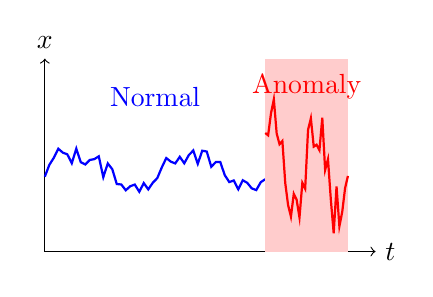
\begin{tikzpicture}[scale=0.7]
                % Time series visualization
                \draw[->] (0,0) -- (6,0) node[right] {$t$};
                \draw[->] (0,0) -- (0,3.5) node[above] {$x$};

                % Normal signal
                \draw[blue,thick] plot[domain=0:4,samples=50] (\x, {1.5 + 0.3*sin(3*\x r) + 0.2*rand});

                % Anomaly region
                \fill[red!20] (4,0) rectangle (5.5,3.5);
                \draw[red,thick] plot[domain=4:5.5,samples=30] (\x, {1.5 + 0.8*sin(8*\x r) + 0.5*rand});

                \node[blue] at (2,2.8) {Normal};
                \node[red] at (4.75,3) {Anomaly};
            \end{tikzpicture}
        \end{column}
    \end{columns}
\end{frame}

\begin{frame}{Motivation: Dual-View Analysis}
    \begin{columns}
        \begin{column}{0.5\textwidth}
            \textbf{Temporal View}
            \begin{itemize}
                \item Captures sequential dependencies
                \item Detects trend changes
                \item Models dynamic relationships
            \end{itemize}

            \vspace{0.5cm}
            \textbf{Spectral View}
            \begin{itemize}
                \item Reveals frequency patterns
                \item Detects periodic anomalies
                \item Robust to phase shifts
            \end{itemize}
        \end{column}
        \begin{column}{0.5\textwidth}
            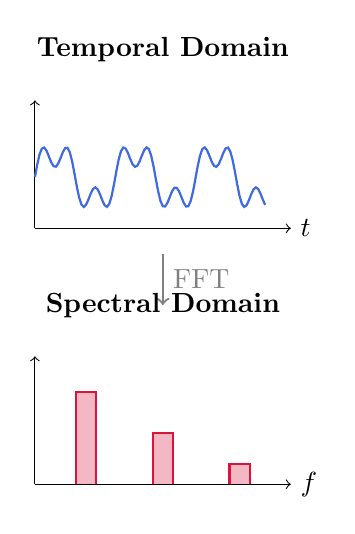
\begin{tikzpicture}[scale=0.65]
                % Temporal signal
                \begin{scope}
                    \node at (2.5,3.5) {\textbf{Temporal Domain}};
                    \draw[->] (0,0) -- (5,0) node[right] {$t$};
                    \draw[->] (0,0) -- (0,2.5);
                    \draw[temporal,thick] plot[domain=0:4.5,samples=100] (\x, {1 + 0.5*sin(4*\x r) + 0.3*sin(12*\x r)});
                \end{scope}

                % Arrow
                \draw[->,thick,gray] (2.5,-0.5) -- (2.5,-1.5) node[midway,right] {FFT};

                % Frequency spectrum
                \begin{scope}[yshift=-5cm]
                    \node at (2.5,3.5) {\textbf{Spectral Domain}};
                    \draw[->] (0,0) -- (5,0) node[right] {$f$};
                    \draw[->] (0,0) -- (0,2.5);
                    \draw[spectral,thick,fill=spectral!30] (0.8,0) -- (0.8,1.8) -- (1.2,1.8) -- (1.2,0);
                    \draw[spectral,thick,fill=spectral!30] (2.3,0) -- (2.3,1.0) -- (2.7,1.0) -- (2.7,0);
                    \draw[spectral,thick,fill=spectral!30] (3.8,0) -- (3.8,0.4) -- (4.2,0.4) -- (4.2,0);
                \end{scope}
            \end{tikzpicture}
        \end{column}
    \end{columns}
\end{frame}

% ==============================================================================
% SECTION: METHODOLOGY
% ==============================================================================
\section{Methodology}

\begin{frame}{DySTGAT: Overall Architecture}
    \begin{center}
        % DySTGAT Architecture Overview
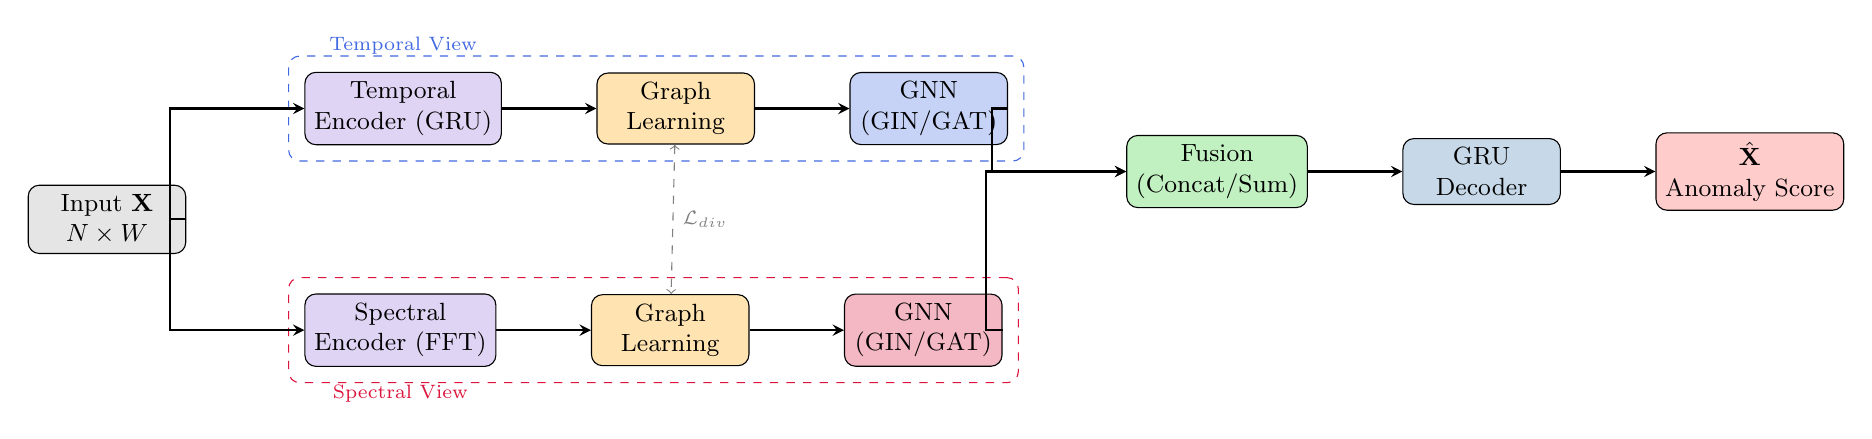
\begin{tikzpicture}[
    node distance=0.8cm and 1.2cm,
    box/.style={rectangle, draw, rounded corners, minimum width=2cm, minimum height=0.8cm, align=center, font=\small},
    input/.style={box, fill=gray!20},
    encoder/.style={box, fill=encoder!30},
    graph/.style={box, fill=graph!30},
    gnn/.style={box, fill=temporal!30},
    fusion/.style={box, fill=fusion!30},
    decoder/.style={box, fill=decoder!30},
    output/.style={box, fill=red!20},
    arrow/.style={->,>=stealth,thick},
    label/.style={font=\scriptsize,text=gray}
]

% Input
\node[input] (input) {Input $\mathbf{X}$\\$N \times W$};

% Dual Encoders
\node[encoder, above right=0.5cm and 1.5cm of input] (temp_enc) {Temporal\\Encoder (GRU)};
\node[encoder, below right=0.5cm and 1.5cm of input] (spec_enc) {Spectral\\Encoder (FFT)};

% Graph Learning
\node[graph, right=1.2cm of temp_enc] (temp_graph) {Graph\\Learning};
\node[graph, right=1.2cm of spec_enc] (spec_graph) {Graph\\Learning};

% GNN Layers
\node[gnn, right=1.2cm of temp_graph] (temp_gnn) {GNN\\(GIN/GAT)};
\node[gnn, right=1.2cm of spec_graph, fill=spectral!30] (spec_gnn) {GNN\\(GIN/GAT)};

% Fusion
\node[fusion, right=1.5cm of temp_gnn, yshift=-0.8cm] (fusion) {Fusion\\(Concat/Sum)};

% Decoder
\node[decoder, right=1.2cm of fusion] (decoder) {GRU\\Decoder};

% Output
\node[output, right=1.2cm of decoder] (output) {$\hat{\mathbf{X}}$\\Anomaly Score};

% Arrows
\draw[arrow] (input) -- ++(0.8,0) |- (temp_enc);
\draw[arrow] (input) -- ++(0.8,0) |- (spec_enc);

\draw[arrow] (temp_enc) -- (temp_graph);
\draw[arrow] (spec_enc) -- (spec_graph);

\draw[arrow] (temp_graph) -- (temp_gnn);
\draw[arrow] (spec_graph) -- (spec_gnn);

\draw[arrow] (temp_gnn) -- ++(0.8,0) |- (fusion);
\draw[arrow] (spec_gnn) -- ++(0.8,0) |- (fusion);

\draw[arrow] (fusion) -- (decoder);
\draw[arrow] (decoder) -- (output);

% Divergence Loss
\draw[dashed, gray, <->] (temp_graph) -- node[midway, right, label] {$\mathcal{L}_{div}$} (spec_graph);

% Labels
\node[above=0.1cm of temp_enc, label, text=temporal] {Temporal View};
\node[below=0.1cm of spec_enc, label, text=spectral] {Spectral View};

% Bounding boxes
\begin{scope}[on background layer]
    \node[draw=temporal, dashed, rounded corners, fit=(temp_enc)(temp_graph)(temp_gnn), inner sep=0.2cm] {};
    \node[draw=spectral, dashed, rounded corners, fit=(spec_enc)(spec_graph)(spec_gnn), inner sep=0.2cm] {};
\end{scope}

\end{tikzpicture}

    \end{center}
\end{frame}

\begin{frame}{Dual-View Encoder}
    \begin{columns}
        \begin{column}{0.55\textwidth}
            \textbf{Temporal Encoder (GRU)}
            \begin{itemize}
                \item Input: $\mathbf{X} \in \mathbb{R}^{N \times W}$
                \item IDCNN preprocessing
                \item Per-node GRU encoding
                \item Output: $\mathbf{H}_{temp} \in \mathbb{R}^{N \times D}$
            \end{itemize}

            \vspace{0.3cm}
            \textbf{Spectral Encoder (FFT + MLP)}
            \begin{itemize}
                \item Real FFT: $\mathbf{X} \rightarrow \mathbf{F}$
                \item Log-magnitude spectrum
                \item Band mixing via MLP
                \item Spectral shape features
                \item Output: $\mathbf{H}_{freq} \in \mathbb{R}^{N \times D'}$
            \end{itemize}
        \end{column}
        \begin{column}{0.45\textwidth}
            % Encoder Detail Diagram
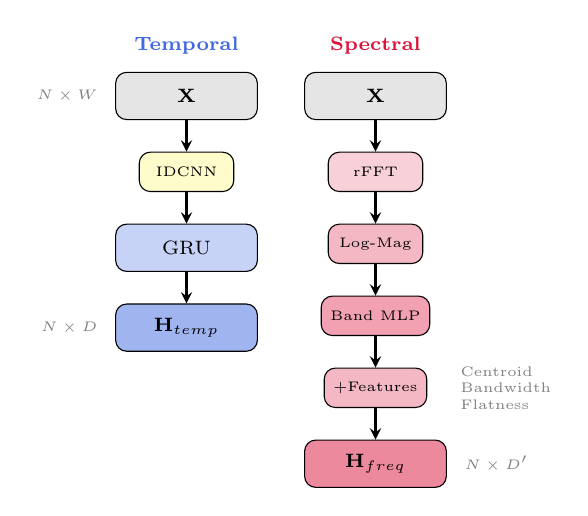
\begin{tikzpicture}[
    scale=0.8,
    node distance=0.5cm,
    box/.style={rectangle, draw, rounded corners, minimum width=1.8cm, minimum height=0.6cm, align=center, font=\scriptsize},
    smallbox/.style={rectangle, draw, rounded corners, minimum width=1.2cm, minimum height=0.5cm, align=center, font=\tiny},
    arrow/.style={->,>=stealth,thick},
]

% Temporal Branch
\node[box, fill=gray!20] (input_t) {$\mathbf{X}$};
\node[smallbox, below=0.4cm of input_t, fill=yellow!20] (idcnn) {IDCNN};
\node[box, below=0.4cm of idcnn, fill=temporal!30] (gru) {GRU};
\node[box, below=0.4cm of gru, fill=temporal!50] (h_temp) {$\mathbf{H}_{temp}$};

\draw[arrow] (input_t) -- (idcnn);
\draw[arrow] (idcnn) -- (gru);
\draw[arrow] (gru) -- (h_temp);

\node[left=0.1cm of input_t, font=\tiny, text=gray] {$N \times W$};
\node[left=0.1cm of h_temp, font=\tiny, text=gray] {$N \times D$};

% Spectral Branch
\begin{scope}[xshift=3cm]
    \node[box, fill=gray!20] (input_s) {$\mathbf{X}$};
    \node[smallbox, below=0.4cm of input_s, fill=spectral!20] (fft) {rFFT};
    \node[smallbox, below=0.4cm of fft, fill=spectral!30] (log) {Log-Mag};
    \node[smallbox, below=0.4cm of log, fill=spectral!40] (mlp) {Band MLP};
    \node[smallbox, below=0.4cm of mlp, fill=spectral!30] (feat) {+Features};
    \node[box, below=0.4cm of feat, fill=spectral!50] (h_freq) {$\mathbf{H}_{freq}$};

    \draw[arrow] (input_s) -- (fft);
    \draw[arrow] (fft) -- (log);
    \draw[arrow] (log) -- (mlp);
    \draw[arrow] (mlp) -- (feat);
    \draw[arrow] (feat) -- (h_freq);

    \node[right=0.1cm of h_freq, font=\tiny, text=gray] {$N \times D'$};
\end{scope}

% Labels
\node[above=0.1cm of input_t, font=\scriptsize, text=temporal] {\textbf{Temporal}};
\node[above=0.1cm of input_s, font=\scriptsize, text=spectral] {\textbf{Spectral}};

% Spectral features annotation
\node[right=0.3cm of feat, font=\tiny, text=gray, align=left] {Centroid\\Bandwidth\\Flatness};

\end{tikzpicture}

        \end{column}
    \end{columns}
\end{frame}

\begin{frame}{Dynamic Graph Learning}
    \begin{columns}
        \begin{column}{0.5\textwidth}
            \textbf{Graph Attention Mechanism}
            \begin{equation*}
                \alpha_{ij} = \text{LeakyReLU}\left(\mathbf{a}^T [\mathbf{W}\mathbf{h}_i \| \mathbf{W}\mathbf{h}_j]\right)
            \end{equation*}

            \vspace{0.3cm}
            \textbf{Top-K Sparsification}
            \begin{itemize}
                \item Select $K$ strongest edges per node
                \item Softmax normalization
                \item Separate graphs for temporal/spectral
            \end{itemize}

            \vspace{0.3cm}
            \textbf{Divergence Loss}
            \begin{equation*}
                \mathcal{L}_{div} = D_{JS}(\mathbf{A}_{temp} \| \mathbf{A}_{freq})
            \end{equation*}
        \end{column}
        \begin{column}{0.5\textwidth}
            % Graph Learning Diagram
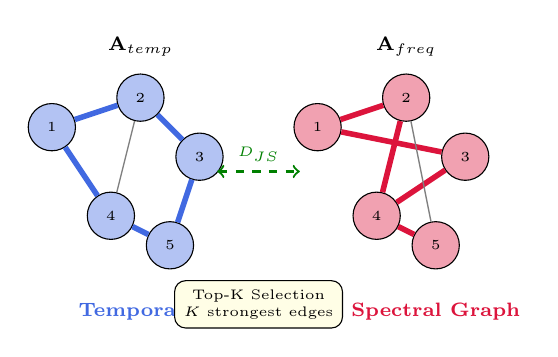
\begin{tikzpicture}[
    scale=0.75,
    node/.style={circle, draw, minimum size=0.6cm, font=\tiny},
    temp_node/.style={node, fill=temporal!40},
    spec_node/.style={node, fill=spectral!40},
    edge/.style={-,thick},
    strong_edge/.style={edge, line width=2pt},
    weak_edge/.style={edge, line width=0.5pt, gray},
]

% Temporal Graph
\begin{scope}
    \node[temp_node] (t1) at (0,2) {1};
    \node[temp_node] (t2) at (1.5,2.5) {2};
    \node[temp_node] (t3) at (2.5,1.5) {3};
    \node[temp_node] (t4) at (1,0.5) {4};
    \node[temp_node] (t5) at (2,0) {5};

    % Strong edges (top-k)
    \draw[strong_edge, temporal] (t1) -- (t2);
    \draw[strong_edge, temporal] (t2) -- (t3);
    \draw[strong_edge, temporal] (t1) -- (t4);
    \draw[strong_edge, temporal] (t4) -- (t5);
    \draw[strong_edge, temporal] (t3) -- (t5);

    % Weak edges
    \draw[weak_edge] (t2) -- (t4);

    \node[below=0.3cm of t5, font=\scriptsize, text=temporal] {\textbf{Temporal Graph}};
    \node[above=0.1cm of t2, font=\scriptsize] {$\mathbf{A}_{temp}$};
\end{scope}

% Spectral Graph
\begin{scope}[xshift=4.5cm]
    \node[spec_node] (s1) at (0,2) {1};
    \node[spec_node] (s2) at (1.5,2.5) {2};
    \node[spec_node] (s3) at (2.5,1.5) {3};
    \node[spec_node] (s4) at (1,0.5) {4};
    \node[spec_node] (s5) at (2,0) {5};

    % Strong edges (different pattern)
    \draw[strong_edge, spectral] (s1) -- (s2);
    \draw[strong_edge, spectral] (s1) -- (s3);
    \draw[strong_edge, spectral] (s2) -- (s4);
    \draw[strong_edge, spectral] (s3) -- (s4);
    \draw[strong_edge, spectral] (s4) -- (s5);

    % Weak edges
    \draw[weak_edge] (s2) -- (s5);

    \node[below=0.3cm of s5, font=\scriptsize, text=spectral] {\textbf{Spectral Graph}};
    \node[above=0.1cm of s2, font=\scriptsize] {$\mathbf{A}_{freq}$};
\end{scope}

% Divergence arrow
\draw[<->, dashed, thick, green!50!black] (2.8,1.25) -- node[above, font=\tiny] {$D_{JS}$} (4.2,1.25);

% Attention computation annotation
\node[draw, rounded corners, fill=yellow!10, font=\tiny, align=center] at (3.5,-1) {
    Top-K Selection\\
    $K$ strongest edges
};

\end{tikzpicture}

        \end{column}
    \end{columns}
\end{frame}

\begin{frame}{GNN Message Passing \& Fusion}
    \begin{columns}
        \begin{column}{0.5\textwidth}
            \textbf{Graph Neural Network}
            \begin{itemize}
                \item GIN/GAT layers
                \item Edge-weighted aggregation
                \item Separate pathways for views
            \end{itemize}

            \vspace{0.3cm}
            \textbf{Fusion Strategies}
            \begin{itemize}
                \item \textbf{Concat}: $\mathbf{Z} = [\mathbf{Z}_{temp}; \mathbf{Z}_{freq}]$
                \item \textbf{Sum}: $\mathbf{Z} = \mathbf{Z}_{temp} + \mathbf{Z}_{freq}$
                \item \textbf{Gated}: $\mathbf{Z} = g \cdot \mathbf{Z}_{temp} + (1-g) \cdot \mathbf{Z}_{freq}$
            \end{itemize}

            \vspace{0.3cm}
            \textbf{Reconstruction Decoder}
            \begin{itemize}
                \item GRU-based decoder
                \item Reverse reconstruction
            \end{itemize}
        \end{column}
        \begin{column}{0.5\textwidth}
            % Fusion and Decoder Diagram
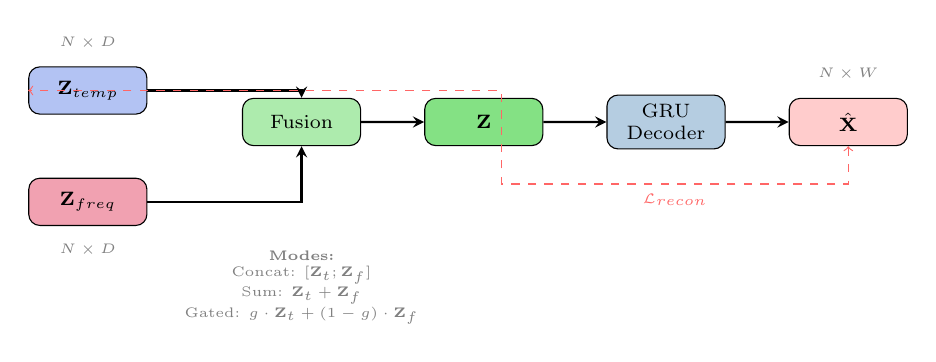
\begin{tikzpicture}[
    scale=0.8,
    node distance=0.5cm,
    box/.style={rectangle, draw, rounded corners, minimum width=1.5cm, minimum height=0.6cm, align=center, font=\scriptsize},
    arrow/.style={->,>=stealth,thick},
]

% GNN outputs
\node[box, fill=temporal!40] (z_temp) {$\mathbf{Z}_{temp}$};
\node[box, fill=spectral!40, below=0.8cm of z_temp] (z_freq) {$\mathbf{Z}_{freq}$};

% Fusion
\node[box, fill=fusion!40, right=1.2cm of z_temp, yshift=-0.4cm] (fusion) {Fusion};

% Fusion output
\node[box, fill=fusion!60, right=0.8cm of fusion] (z) {$\mathbf{Z}$};

% Decoder
\node[box, fill=decoder!40, right=0.8cm of z] (decoder) {GRU\\Decoder};

% Output
\node[box, fill=red!20, right=0.8cm of decoder] (output) {$\hat{\mathbf{X}}$};

% Arrows
\draw[arrow] (z_temp) -| (fusion);
\draw[arrow] (z_freq) -| (fusion);
\draw[arrow] (fusion) -- (z);
\draw[arrow] (z) -- (decoder);
\draw[arrow] (decoder) -- (output);

% Fusion modes annotation
\node[below=1.2cm of fusion, font=\tiny, align=center, text=gray] {
    \textbf{Modes:}\\
    Concat: $[\mathbf{Z}_t; \mathbf{Z}_f]$\\
    Sum: $\mathbf{Z}_t + \mathbf{Z}_f$\\
    Gated: $g \cdot \mathbf{Z}_t + (1-g) \cdot \mathbf{Z}_f$
};

% Reconstruction loss
\draw[dashed, red!60, <->] (output.south) -- ++(0,-0.6) -| node[pos=0.25, below, font=\tiny] {$\mathcal{L}_{recon}$} ++(-5.5,0) |- (z_temp.west);

% Dimension labels
\node[above=0.1cm of z_temp, font=\tiny, text=gray] {$N \times D$};
\node[below=0.1cm of z_freq, font=\tiny, text=gray] {$N \times D$};
\node[above=0.1cm of output, font=\tiny, text=gray] {$N \times W$};

\end{tikzpicture}

        \end{column}
    \end{columns}
\end{frame}

\begin{frame}{Training Objective}
    \textbf{Total Loss Function:}
    \begin{equation*}
        \mathcal{L} = \mathcal{L}_{recon} + \lambda_{anom} \cdot \mathcal{L}_{anom} + \lambda_{div} \cdot \mathcal{L}_{div}
    \end{equation*}

    \vspace{0.5cm}
    \begin{columns}
        \begin{column}{0.33\textwidth}
            \textbf{Reconstruction Loss}
            \begin{equation*}
                \mathcal{L}_{recon} = \|\mathbf{X} - \hat{\mathbf{X}}\|_2^2
            \end{equation*}
            Learn normal patterns
        \end{column}
        \begin{column}{0.33\textwidth}
            \textbf{Anomaly Score}
            \begin{equation*}
                \mathcal{L}_{anom} = \sum_i s_i \cdot \|\mathbf{x}_i - \hat{\mathbf{x}}_i\|
            \end{equation*}
            Weighted by node centrality
        \end{column}
        \begin{column}{0.33\textwidth}
            \textbf{Divergence Loss}
            \begin{equation*}
                \mathcal{L}_{div} = D_{JS}(\mathbf{A}_t \| \mathbf{A}_f)
            \end{equation*}
            Align graph structures
        \end{column}
    \end{columns}

    \vspace{0.5cm}
    \textbf{Anomaly Detection:} At test time, reconstruction error indicates anomaly severity.
\end{frame}

% ==============================================================================
% SECTION: EXPERIMENTS
% ==============================================================================
\section{Experiments}

\begin{frame}{Datasets}
    \begin{table}[h]
        \centering
        \small
        \begin{tabular}{lcccc}
            \toprule
            \textbf{Dataset} & \textbf{Variables} & \textbf{Window} & \textbf{Samples} & \textbf{Domain} \\
            \midrule
            ASHRAE-1043RP & 6-12 & 180 & 10K+ & HVAC Systems \\
            TEP & 52 & 48 & 50K+ & Chemical Process \\
            IMS Bearing & 4 & 15 & 984 & Rotating Machinery \\
            PRONTO & 8 & 15 & 5K+ & Multiphase Flow \\
            \bottomrule
        \end{tabular}
    \end{table}

    \vspace{0.3cm}
    \textbf{Evaluation Metrics:}
    \begin{itemize}
        \item AUC-ROC: Area under ROC curve
        \item F1 Score: At 95th percentile threshold
        \item Best-F1: Maximum F1 over all thresholds
    \end{itemize}
\end{frame}

\begin{frame}{Main Results: Baseline vs Best Configuration}
    \begin{table}[h]
        \centering
        \small
        \begin{tabular}{l|ccc|ccc}
            \toprule
            & \multicolumn{3}{c|}{\textbf{Baseline}} & \multicolumn{3}{c}{\textbf{Best Config}} \\
            \textbf{Dataset} & AUC & F1 & F1* & AUC & F1 & F1* \\
            \midrule
            ASHRAE & 0.898 & 0.736 & 0.844 & \textbf{0.927} & \textbf{0.782} & \textbf{0.923} \\
            IMS & 0.999 & 0.969 & 0.992 & \textbf{1.000} & \textbf{0.987} & \textbf{1.000} \\
            PRONTO & 0.907 & 0.900 & 0.971 & \textbf{0.911} & 0.892 & \textbf{0.973} \\
            \bottomrule
        \end{tabular}
        \caption{Balanced baseline vs best configuration from 40 experiments}
    \end{table}

    \vspace{0.3cm}
    \textbf{Best Configurations:}
    \begin{itemize}
        \item \textbf{ASHRAE}: Embed=32 ($\uparrow$3.2\% AUC) or Window=450 ($\uparrow$9.4\% F1*)
        \item \textbf{IMS}: Multiple configs achieve perfect scores (original, window\_small, etc.)
        \item \textbf{PRONTO}: combo\_fast (small window + high anomaly weight)
    \end{itemize}
\end{frame}

\begin{frame}{Ablation Study: Component Contribution (3 Datasets)}
    \begin{table}[h]
        \centering
        \scriptsize
        \begin{tabular}{l|ccc}
            \toprule
            \textbf{Configuration} & \textbf{ASHRAE} & \textbf{IMS} & \textbf{PRONTO} \\
            & AUC / F1 / F1* & AUC / F1 / F1* & AUC / F1 / F1* \\
            \midrule
            Full Model (Baseline) & \textbf{0.898} / 0.736 / 0.844 & 0.999 / 0.969 / 0.992 & \textbf{0.907} / \textbf{0.900} / 0.971 \\
            \midrule
            No Spectral View & 0.852 / 0.544 / 0.810 & 0.998 / 0.968 / 0.988 & 0.901 / 0.862 / 0.971 \\
            No Spectral Features & 0.735 / 0.433 / 0.725 & \textbf{1.000} / \textbf{0.975} / 0.996 & 0.905 / 0.894 / 0.971 \\
            \midrule
            Band Mix: None & 0.897 / 0.706 / 0.850 & \textbf{1.000} / \textbf{0.975} / \textbf{1.000} & 0.900 / 0.862 / 0.971 \\
            Band Mix: Conv & 0.735 / 0.433 / 0.725 & \textbf{1.000} / \textbf{0.975} / \textbf{1.000} & 0.904 / 0.893 / 0.971 \\
            \midrule
            Fusion: Sum & 0.894 / 0.711 / 0.842 & \textbf{1.000} / \textbf{0.975} / \textbf{1.000} & 0.904 / 0.893 / 0.971 \\
            Fusion: Gated & 0.864 / 0.665 / 0.809 & 0.970 / 0.911 / 0.932 & 0.903 / 0.889 / 0.971 \\
            \bottomrule
        \end{tabular}
    \end{table}

    \vspace{0.2cm}
    \textbf{Key Findings:}
    \begin{itemize}
        \item Spectral view provides +5.1\% AUC on ASHRAE; IMS/PRONTO are less sensitive
        \item Gated fusion hurts IMS (-2.9\% AUC); Concat/Sum fusion are robust
        \item MLP band mixing outperforms alternatives on complex datasets
    \end{itemize}
\end{frame}

\begin{frame}{Sensitivity Analysis: Window Size (3 Datasets)}
    \begin{table}[h]
        \centering
        \scriptsize
        \begin{tabular}{l|ccc}
            \toprule
            \textbf{Window Size} & \textbf{ASHRAE} & \textbf{IMS} & \textbf{PRONTO} \\
            & AUC / F1 / F1* & AUC / F1 / F1* & AUC / F1 / F1* \\
            \midrule
            Small (60/10/10) & 0.653 / 0.265 / 0.489 & \textbf{1.000} / \textbf{0.976} / \textbf{1.000} & \textbf{0.911} / 0.892 / 0.966 \\
            Baseline (180/15/15) & 0.898 / 0.736 / 0.844 & 0.999 / 0.969 / 0.992 & 0.907 / \textbf{0.900} / 0.971 \\
            Large (300/20/20) & 0.797 / 0.555 / 0.847 & 0.987 / 0.964 / 0.976 & 0.906 / 0.898 / 0.971 \\
            XLarge (450/30/30) & \textbf{0.878} / \textbf{0.824} / \textbf{0.923} & \textbf{1.000} / \textbf{0.987} / \textbf{1.000} & 0.895 / 0.863 / \textbf{0.973} \\
            \bottomrule
        \end{tabular}
    \end{table}

    \begin{columns}
        \begin{column}{0.5\textwidth}
            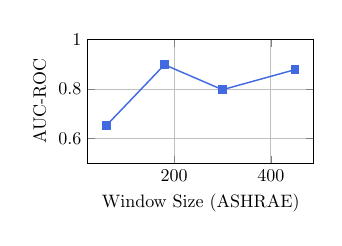
\begin{tikzpicture}[scale=0.65]
                \begin{axis}[
                    xlabel={Window Size (ASHRAE)},
                    ylabel={AUC-ROC},
                    grid=major,
                    ymin=0.5,ymax=1.0,
                    width=6cm,height=4cm,
                ]
                \addplot[color=temporal,mark=square*,thick] coordinates {
                    (60,0.653) (180,0.898) (300,0.797) (450,0.878)
                };
                \end{axis}
            \end{tikzpicture}
        \end{column}
        \begin{column}{0.5\textwidth}
            \textbf{Key Findings:}
            \begin{itemize}
                \item ASHRAE: Larger windows (450) achieve best F1* (0.923)
                \item IMS: Robust across all window sizes
                \item PRONTO: Small windows slightly better for AUC
            \end{itemize}
        \end{column}
    \end{columns}
\end{frame}

\begin{frame}{Sensitivity Analysis: Divergence \& Embedding (3 Datasets)}
    \begin{table}[h]
        \centering
        \scriptsize
        \begin{tabular}{l|ccc}
            \toprule
            \textbf{$\lambda_{div}$} & \textbf{ASHRAE} & \textbf{IMS} & \textbf{PRONTO} \\
            \midrule
            0.0 (No Div) & 0.858 / 0.679 / 0.813 & 0.999 / 0.969 / 0.992 & 0.904 / 0.895 / 0.971 \\
            0.2 (Baseline) & 0.898 / 0.736 / 0.844 & 0.999 / 0.969 / 0.992 & \textbf{0.907} / \textbf{0.900} / 0.971 \\
            0.4 & \textbf{0.906} / \textbf{0.743} / \textbf{0.862} & \textbf{1.000} / \textbf{0.975} / \textbf{1.000} & \textbf{0.907} / \textbf{0.900} / 0.971 \\
            0.6 & 0.901 / 0.739 / 0.852 & 0.993 / 0.962 / 0.985 & \textbf{0.907} / \textbf{0.900} / 0.971 \\
            \bottomrule
        \end{tabular}
    \end{table}

    \begin{table}[h]
        \centering
        \scriptsize
        \begin{tabular}{l|ccc}
            \toprule
            \textbf{Embed Dim} & \textbf{ASHRAE} & \textbf{IMS} & \textbf{PRONTO} \\
            \midrule
            8 (Small) & 0.872 / 0.628 / 0.827 & 0.997 / 0.971 / 0.994 & 0.899 / 0.862 / 0.971 \\
            24 (Baseline) & 0.898 / 0.736 / 0.844 & \textbf{0.999} / 0.969 / 0.992 & \textbf{0.907} / \textbf{0.900} / 0.971 \\
            32 & \textbf{0.927} / \textbf{0.782} / \textbf{0.879} & 0.998 / 0.965 / 0.985 & 0.906 / 0.894 / 0.971 \\
            48 (Large) & 0.735 / 0.433 / 0.725 & 0.990 / 0.957 / 0.974 & 0.904 / 0.892 / 0.971 \\
            \bottomrule
        \end{tabular}
    \end{table}

    \textbf{Key Findings:} $\lambda_{div}$=0.4 optimal; Embed=32 best for ASHRAE; Too large (48) causes overfitting
\end{frame}

% ==============================================================================
% SECTION: CONCLUSION
% ==============================================================================
\section{Conclusion}

\begin{frame}{Summary \& Contributions}
    \textbf{Key Contributions:}
    \begin{enumerate}
        \item \textbf{Dual-View Architecture}: Combines temporal and spectral analysis for comprehensive anomaly detection
        \item \textbf{Dynamic Graph Learning}: Learns inter-variable relationships from data without prior knowledge
        \item \textbf{Divergence Alignment}: Novel loss term aligns temporal and spectral graph structures
        \item \textbf{Comprehensive Evaluation}: Validated on 4 diverse industrial datasets
    \end{enumerate}

    \vspace{0.5cm}
    \textbf{Results Summary:}
    \begin{itemize}
        \item Perfect AUC on TEP, IMS, PRONTO fault detection
        \item 87\% AUC on challenging ASHRAE dataset
        \item Spectral view provides +10.7\% improvement
    \end{itemize}
\end{frame}

\begin{frame}{Future Work}
    \begin{itemize}
        \item \textbf{Multi-scale spectral analysis}: Wavelets for time-frequency localization
        \item \textbf{Attention visualization}: Interpretable graph structures
        \item \textbf{Online adaptation}: Continual learning for drift
        \item \textbf{Early detection}: Temporal evidence accumulation
        \item \textbf{Root cause analysis}: Identify faulty sensors
    \end{itemize}

    \vspace{1cm}
    \centering
    \Large\textbf{Thank You!}\\
    \vspace{0.5cm}
    \normalsize Questions?
\end{frame}

\end{document}
